% ------------------------------------------------------------------------------
% TYPO3 v9 LTS - What's New (German Version)
%
% @license	Creative Commons BY-NC-SA 3.0
% @link		https://typo3.org/help/documentation/whats-new/
% @language	German
% ------------------------------------------------------------------------------

\section{Einführung}
\begin{frame}[fragile]
	\frametitle{Einführung}

	\begin{center}\huge{\color{typo3darkgrey}\textbf{Einführung}}\end{center}
	\begin{center}\large{\textit{Wichtige Fakten und Zahlen}}\end{center}

\end{frame}

% ------------------------------------------------------------------------------
% TYPO3 CMS 9 LTS - The Facts

\begin{frame}[fragile]
	\frametitle{Einführung}
	\framesubtitle{TYPO3 v9 LTS}

	\begin{itemize}
		\item Veröffentlichungsdatum: 2. Oktober 2018
		\item Releasetyp: LTS Release (Long Term Release)
		\item Entwicklungszeit: 18 Monate
	\end{itemize}

	\begin{figure}
		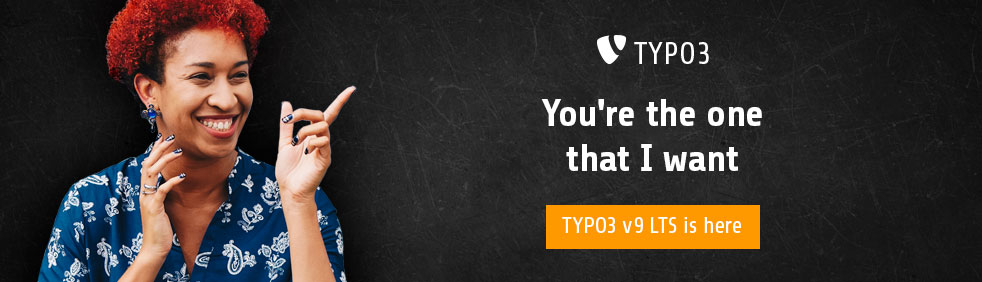
\includegraphics[width=0.95\linewidth]{Introduction/typo3-v95-banner.jpg}
	\end{figure}

\end{frame}

% ------------------------------------------------------------------------------
% System Requirements

\begin{frame}[fragile]
	\frametitle{Einführung}
	\framesubtitle{Systemvoraussetzungen}

	\begin{itemize}
		\item PHP Version 7.2+
		\item PHP Einstellungen:

			\begin{itemize}
				\item \texttt{memory\_limit} >= 256M
				\item \texttt{max\_execution\_time} >= 240s
				\item \texttt{max\_input\_vars} >= 1500
				\item Die Option \texttt{-}\texttt{-disable-ipv6} darf \underline{nicht} gesetzt sein
			\end{itemize}

		\item Erforderliche PHP-Erweiterungen:\newline
			\small
				filter, hash, openssl, pcre >= 8.38, session, SPL, standard,
				xml, zip and zlib
			\normalsize
	\end{itemize}

\end{frame}

% ------------------------------------------------------------------------------
% System Requirements

\begin{frame}[fragile]
	\frametitle{Einführung}
	\framesubtitle{Systemvoraussetzungen}

	\begin{itemize}
		\item Webserver wie Apache, Nginx, IIS, usw.
		\item Von \textbf{Doctrine DBAL} unterstützte Datenbanken werden ebenfalls
			von TYPO3 unterstützt. Beispielsweise:
	\end{itemize}

	\begin{figure}
		
\includegraphics[width=0.70\linewidth]{Introduction/logo-databases.png}
	\end{figure}

	\begin{itemize}
		\item Festplattenplatz: mindestens 200 MB
		\item Das Backend benötigt Microsoft Internet Explorer 11 oder höher,
			Microsoft Edge, Google Chrome, Firefox, Safari oder jeden anderen
			modernen Browser
	\end{itemize}

\end{frame}

% ------------------------------------------------------------------------------
% Sprint Releases

\begin{frame}[fragile]
	\frametitle{Einführung}
	\framesubtitle{Release Zyklus}

	Sprint Releases veröffentlicht:

	\begin{itemize}
		\item v9.0 \tabto{1.1cm}12/Dec/2017\tabto{3.4cm}Install Tool und Page Tree Refactoring,\newline
			\tabto{3.4cm}Vereinheitlichte Seitenübersetzungen
		\item v9.1 \tabto{1.1cm}30/Jan/2018\tabto{3.4cm}Redirect Handling
		\item v9.2 \tabto{1.1cm}10/Apr/2018\tabto{3.4cm}Site Handling
		\item v9.3 \tabto{1.1cm}12/Jun/2018\tabto{3.4cm}SEO und URL Routing Vorbereitungen
		\item v9.4 \tabto{1.1cm}04/Sep/2018\tabto{3.4cm}URL-Routing für Seiten
		\item v9.5 \tabto{1.1cm}02/Oct/2018\tabto{3.4cm}LTS Vorbereitung und Release
	\end{itemize}

\end{frame}

% ------------------------------------------------------------------------------
% LTS Support Timeline

\begin{frame}[fragile]
	\frametitle{Einführung}
	\framesubtitle{Long Term Support}

	\begin{figure}
		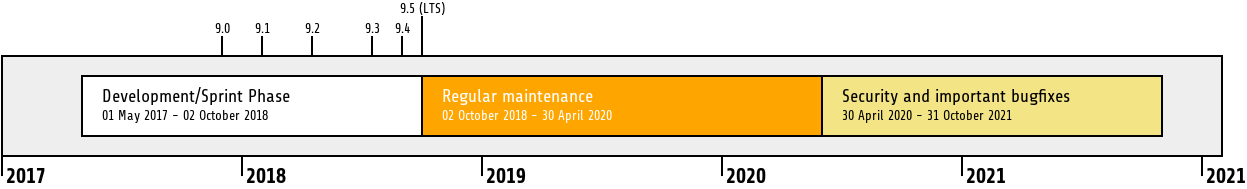
\includegraphics[width=1\linewidth]{Introduction/typo3-v9-lifecycle.png}
	\end{figure}

	\begin{itemize}
		\item TYPO3 Version 9.5 ist eine LTS-Version (Long Term Support)
		\item Instandhaltung und Bugfixes bis März 2020
		\item Sicherheitsthemen und kritische Bugfixes bis Oktober 2021
	\end{itemize}
	\vspace{0.2cm}
	\textbf{Erweiterte Unterstützung}\newline
	\smaller
		\href{https://typo3.com} Die {TYPO3 GmbH} bietet erweiterte Unterstützung
			(ELTS) für TYPO3 v9 LTS bis Oktober 2024.
	\normalsize

\end{frame}

% ------------------------------------------------------------------------------
